\documentclass[conference]{IEEEtran}
\IEEEoverridecommandlockouts
% The preceding line is only needed to identify funding in the first footnote. If that is unneeded, please comment it out.
\usepackage{cite}
\usepackage{amsmath,amssymb,amsfonts}
\usepackage{algorithmic}
\usepackage{graphicx}
\usepackage{textcomp}
\usepackage{xcolor}
\usepackage{hhline}
\def\BibTeX{{\rm B\kern-.05em{\sc i\kern-.025em b}\kern-.08em
    T\kern-.1667em\lower.7ex\hbox{E}\kern-.125emX}}
\begin{document}

\title{An Efficient and Implementation-friendly Method for More Smart ADCs' Design in Edge Computing with Dynamical Energy Optimization\\}
%An Efficient and Implementation-friendly ADC extension Method with Precision Adaptive and Fine-grained Power Management Strategies for More Intelligent Edge Computing Scenarios

\author{\IEEEauthorblockN{1\textsuperscript{st} Given Name Surname}
\IEEEauthorblockA{\textit{dept. name of organization (of Aff.)} \\
\textit{name of organization (of Aff.)}\\
City, Country \\
email address or ORCID}
\and
\IEEEauthorblockN{2\textsuperscript{nd} Given Name Surname}
\IEEEauthorblockA{\textit{dept. name of organization (of Aff.)} \\
\textit{name of organization (of Aff.)}\\
City, Country \\
email address or ORCID}
\and
\IEEEauthorblockN{3\textsuperscript{rd} Given Name Surname}
\IEEEauthorblockA{\textit{dept. name of organization (of Aff.)} \\
\textit{name of organization (of Aff.)}\\
City, Country \\
email address or ORCID}
\and
\IEEEauthorblockN{4\textsuperscript{th} Given Name Surname}
\IEEEauthorblockA{\textit{dept. name of organization (of Aff.)} \\
\textit{name of organization (of Aff.)}\\
City, Country \\
email address or ORCID}
\and
\IEEEauthorblockN{5\textsuperscript{th} Given Name Surname}
\IEEEauthorblockA{\textit{dept. name of organization (of Aff.)} \\
\textit{name of organization (of Aff.)}\\
City, Country \\
email address or ORCID}
\and
\IEEEauthorblockN{6\textsuperscript{th} Given Name Surname}
\IEEEauthorblockA{\textit{dept. name of organization (of Aff.)} \\
\textit{name of organization (of Aff.)}\\
City, Country \\
email address or ORCID}
}

\maketitle

\begin{abstract}
As precision adaptive computing has already been widely studied for more efficeint Neural Networks (NNs), Analog-to-Digital Converters (ADCs), which dominate the power consumption of traditional sensing systems, can also be smartly designed for more intelligent edge computing. In this work, we propose a method combining adaptive precision and fine-grained power management strategies for more smart ADCs' design with dynamical energy optimization. We present two case study ADC designs and demonstrate the effectiveness of the proposed method in detail. Results show that almost a half of the ADCs’ power consumption can be reduced in the low precision mode, while the cost of extra control circuits is rather small. As this method is easy to resonate with multiple downstream algorithms, it will be promising for ultra-efficient edge computing in the future.
\end{abstract}

\begin{IEEEkeywords}
ADC, precision adaptive, power management, energy-efficient, edge computing
\end{IEEEkeywords}

\section{Introduction}

With the development of the Internet-of-Things (IoT), edge devices like mobile phones, smart watches, and other portable products have been playing an important role in people’s daily lives for collecting and processing data in site and in time. On the other hand, Neural Networks have shown broad prospects for sensing applications, such as computer vision, speech recognition, and robotics. Therefore, deploying NNs on edge devices is an emerging trend which leads to many efforts of research. 

To integrate large and computationally intensive NN models on edge devices of which the power supply and computing resources are quite limited, improving the systems' energy efficiency is critical. While compression and optimization of NN models have been extensively studied [xxxx], Analog-to-Digital Converters, which dominate the power consumption of traditional sensing systems, have been generally treated as black boxes. 

However, as more and more intelligent algorithms are able to process data of varying precision for different tasks[xxxx], opportunities have been offered for us to achieve better energy efficiency by taking algorithm-aware adjustments inside the ADCs. Considering the precision (i.e. the quantization bits) is at the heart of an ADC’s energy constraints, making it dynamically adaptive will be promising.

In certain applications, such as image processing, the camera’s resolution has already been considered to be dynamically adaptive for efficient multi-task analysis [xxxx], where the precision of ADCs has not been considered as a variable. Besides, there are efforts trying to relieve the design specifications of ADCs by applying low-precision analog computing firstly close to the sensor [xxxx]. But high-precision ADCs and NN processors are still there for complex tasks. Therefore, dynamical energy optimization inside ADCs remains competitive.

Motivated by these facts, we mainly makes the following contributions in this paper:
\begin{enumerate}[\IEEEsetlabelwidth{3)}]
	\item A method combining adaptive precision and power gating is proposed for more smart ADCs' design with dynamicall energy optimization. With the fine-grained power management strategies, which have rarely been studied before, we successfully reduce the ADCs' power consumptionin to nearly half in the low-precision mode.
	\item Two case study ADC designs are presented. The first one is column-parallel Single-Slope (SS) ADCs and the second is column-parallel SAR/SS ADCs. We analyze the power distribution of the ADCs in detail and demonstrate the effectiveness of the proposed method with specific simulating results. Both of the two designs can be applied in the CMOS Image Sensors (CISs) and are suitable for different design specifications. 
	\item As the evaluation results are easy to extend and the extra control logic is implementation-friendly, we argue for the universality of the proposed method for ADCs of not only different architectures but also varying application scenarios.
\end{enumerate} 

The remainder of this paper is organized as follows. Sect.~\ref{architecture} presents the architecture overview of the two case study ADC designs. Sect.~\ref{strategy} describes the adaptive precision and power gating strategies for the two case study ADC designs, specifically. Sect.~\ref{result} reports the evaluation results and Sect.~\ref{discussion} develops discussions. Finally, Sect.~\ref{conclusion} concludes this paper.

\section{Architecture Overview}\label{architecture}

\subsection{Architecture of the SS ADCs}

The overall architecture of the SS ADCs is presented in Fig.~\ref{SSADC}. The main modules include column-parallel Correlated Double Sampling (CDS) circuits, comparators, and a column-shared ramp generator. Fig.~\ref{SSWAVE} shows the basic operational waveform of the SS ADCs. When the ramp signal exceeds the output of a CDS circuit in a certain column, the corresponding comparator will be flipped and latch the time information $\Delta t$ in the 8-bit registers in that column as conversion results. And Such conversions across all columns will be done as soon as the ramp signal reaches $V_{refh}$.
\begin{figure}[htbp]
	\centerline{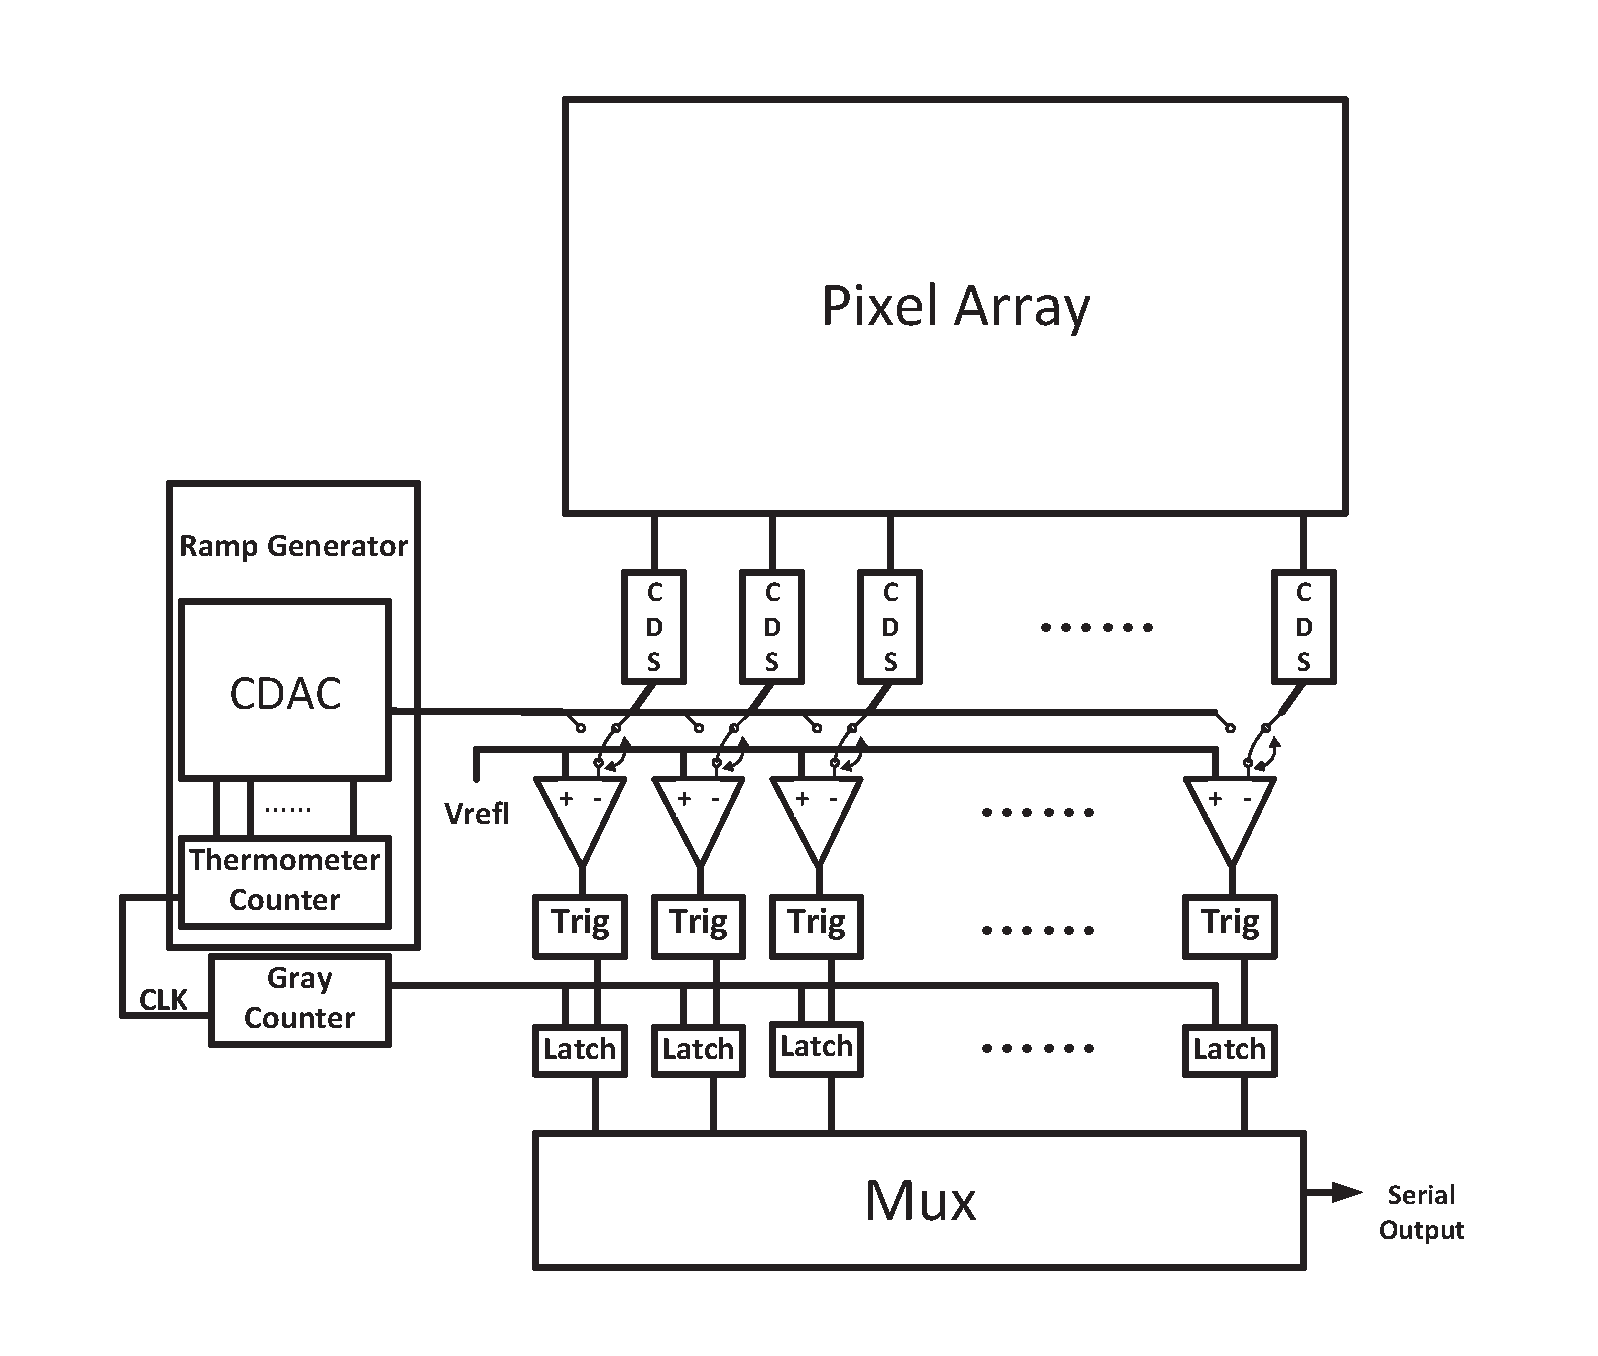
\includegraphics[width=3.5in]{./Figures/SSADC.eps}}
	\caption{Overall Architecture of the SS ADCs.}
	\label{SSADC}
\end{figure} 
\begin{figure}[htbp]
	\centerline{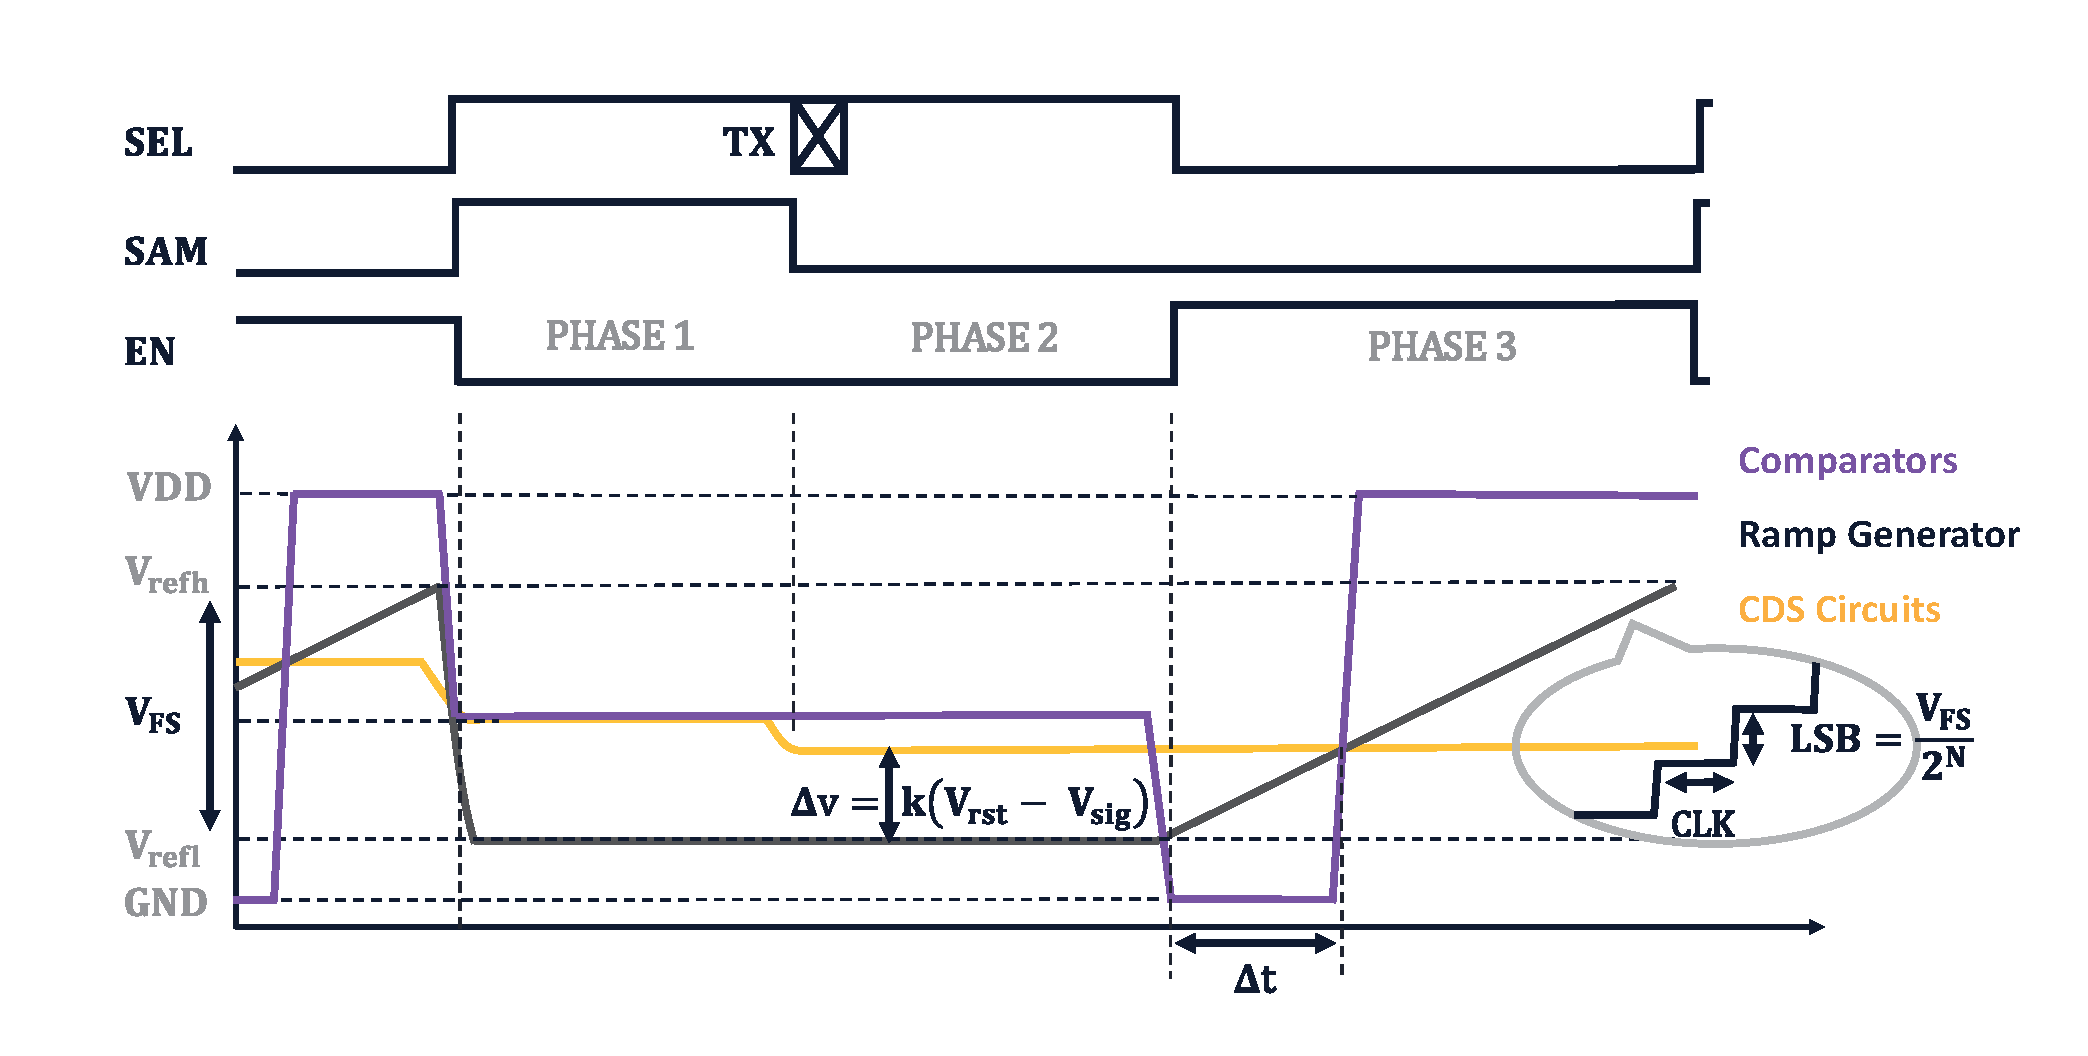
\includegraphics[width=3.5in]{./Figures/SSWAVE.eps}}
	\caption{Operational waveform of the SS ADCs.}
	\label{SSWAVE}
\end{figure}

As the structure of the three main modules are described more specifically as follows, details of the three waves in Fig.~\ref{SSWAVE} are also revealed.

\subsubsection{CDS Circuits}

CDS circuits are the interface between the pixel array and the ADCs, responsible for subtracting the pixels’ signal voltages from reference voltages and amplifying the difference by a certain coefficient. The difference (i.e. $\Delta{V}$ in Fig.~\ref{SSWAVE}) is physically attached to the exposure time of the pixels, and the subtraction will help cancel the noises caused by the varying reference voltages. 

Switched-capacitor operational amplifiers are commonly used in CDS circuits as presented in Fig.~\ref{CDS}. According to the law of charge conservation, the output voltage of the CDS circuits (in PHASE2 of Fig.~\ref{SSWAVE}) can be calculated as \eqref{eq1}. It is noticed that the Input Offset Cancelation (IOS) is realized, which is necessary because the amplifiers in different columns may have different offset voltage.
\begin{figure}[htbp]
	\centerline{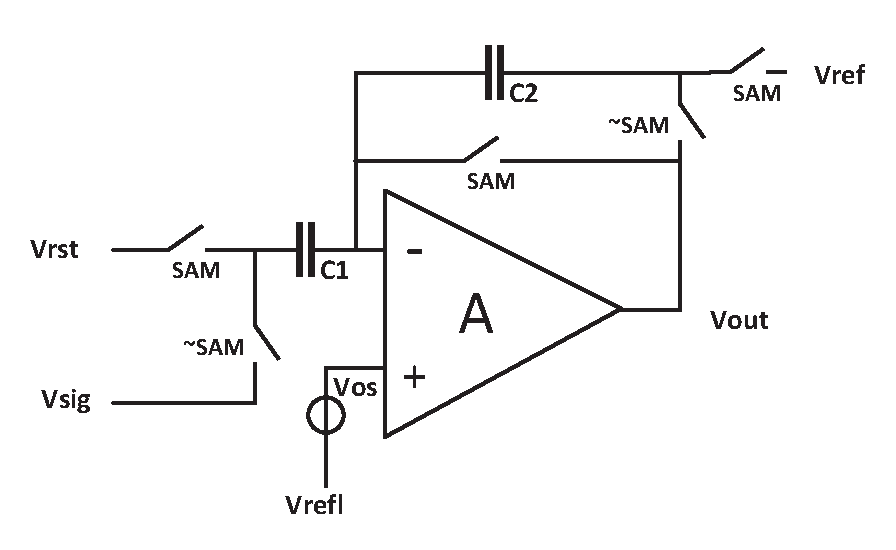
\includegraphics[width=2.5in]{./Figures/CDS.eps}}
	\caption{the Structure of the CDS Circuits.}
	\label{CDS}
\end{figure} 
\begin{equation}
\begin{aligned}
	V_{out}&=\left[ V_{ref}+\frac{C_1}{C_2}\ast\left(V_{rst}-V_{sig}\right)\right]\ast\frac{\beta A}{1+\beta A}\\
	 &\;{+}\;\left(V\right._{refl}+V_{os})\ast\frac{A}{1+A}\ast\frac{1}{\beta A}\\
	 &\;where\ \ \beta=\frac{C_2}{C_1+C_2}
	\label{eq1}
\end{aligned}
\end{equation}

\subsubsection{the Ramp Generater}

As presented in Fig.~\ref{RAMP}, the ramp generator consists of a thermometer counter and a Capacitor Digital-to-Analog Converter (CDAC). While the capacitors in CDAC are being switched one by one from $V_{refl}$ to $V_{vefh}$, the output voltage of the ramp generator will be as \eqref{eq2} according to the law of charge conservation. In this equation, $N$ means the number of switched capacitors and $M$ means the total number of capacitors of the same size (for the 8-bit precision, the total number will be 255). Therefore, as in PHASE3 of Fig.~\ref{SSWAVE}, the ramp signal will be like stages from $V_{refl}$ to $V_{refh}$, of which the range is consistent with the output of CDS circuits. And the height of every stage is actually the Least Significant Bit (LSB) converted by the ADCs.
 
The three buffers in Fig.~\ref{RAMP} make sure that the reference voltages and ramp signal have enough driving capability, and the output buffer will be in the largest size because it has to drive hundreds of column-parallel comparators.
\begin{figure}[htbp]
	\centerline{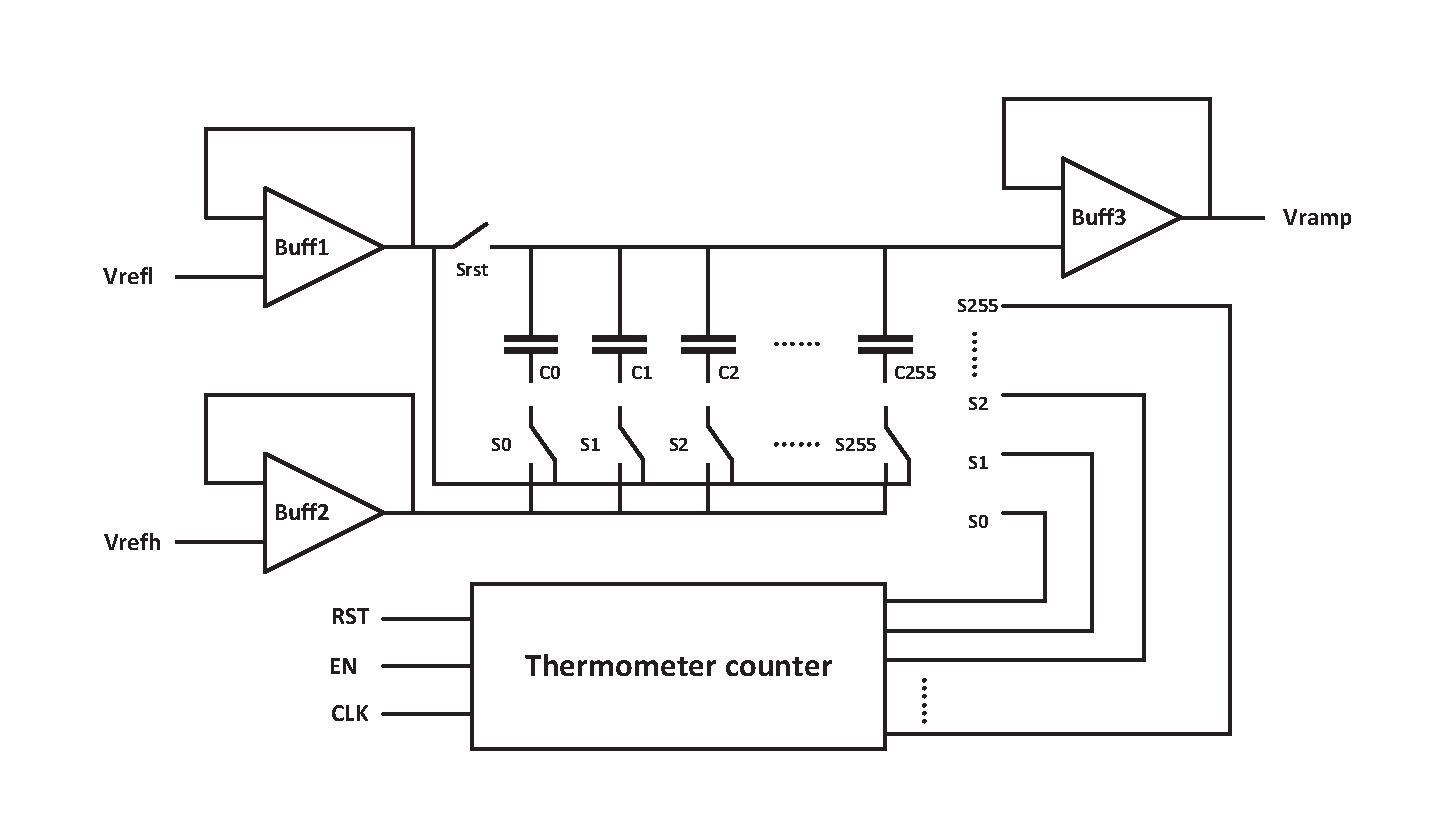
\includegraphics[width=3.5in]{./Figures/RAMP.eps}}
	\caption{the Structure of the Ramp Generator.}
	\label{RAMP}
\end{figure} 
\begin{equation}
	V_{ramp}=V_{refl}+\frac{N}{M}\ast\left(V_{refh}-V_{refl}\right)
		\label{eq2}
\end{equation}
\subsubsection{Comparators}
The comparators work for comparing the CDS circuits' output and the ramp signal. In the SS ADCs, two-stage open-loop comparators can be applied as presented in Fig.~\ref{COM}. Again according to the law of charge conservation, the comparators’ output (in PHASE3 of Fig.~\ref{SSWAVE}) can be calculated as \eqref{eq3}. The comparison will be dominated by $V_{ramp}-V_{cds}$ as long as the amplifiers’ open-loop gain is large enough and the IOS is realized. Besides, the comparators’ speed depends on the amplifiers’ bandwidth and slew rate.
\begin{figure}[htbp]
	\centerline{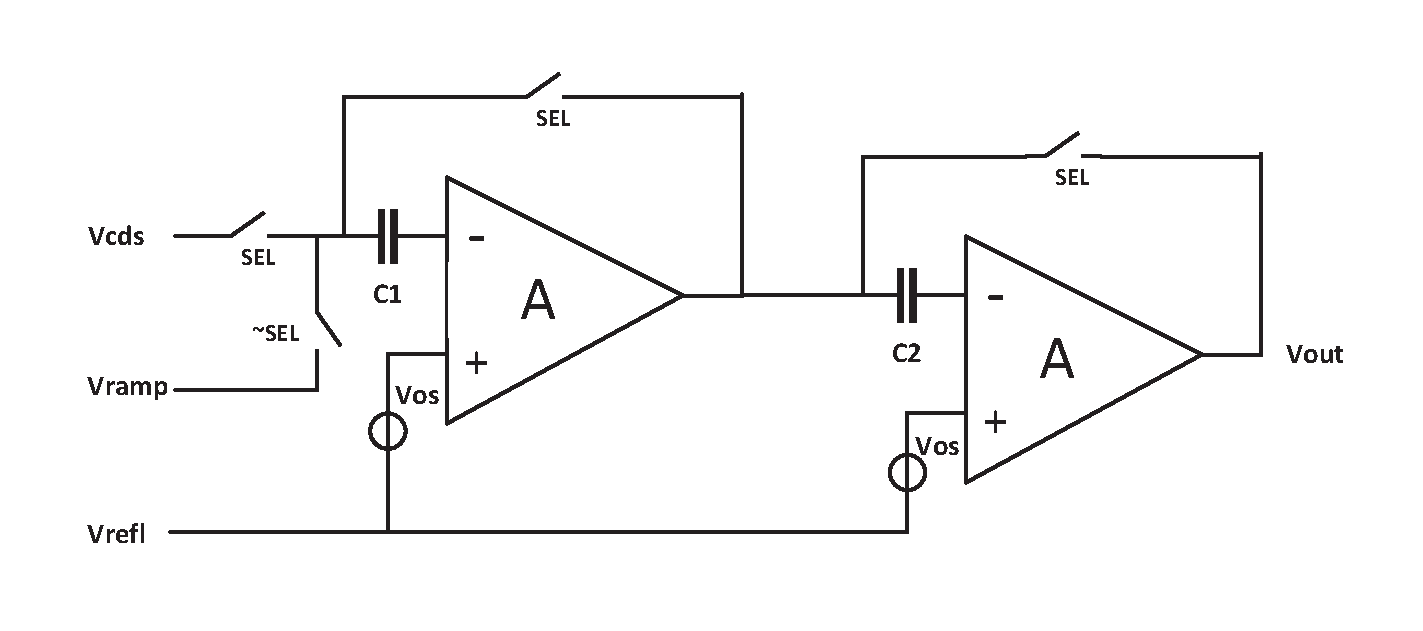
\includegraphics[width=3.5in]{./Figures/COM.eps}}
	\caption{the Structure of the Comparators in the SS ADCs.}
	\label{COM}
\end{figure} 
\begin{equation}
	\begin{aligned}
		V_{out}&=A^2(V_{ramp}-V_{cds})\\
		&\;{+}\;\left(V_{refl}+V_{os}\right)\ast\frac{A}{1+A}\\ 		
		\label{eq3}
	\end{aligned}
\end{equation}

\subsection{Architecture of the SAR/SS ADCs}

The overall architecture of the SAR/SS ADCs is almost the same as the SS ADCs, and the only difference is that the comparators are now replaced with low-precision (4bit) SAR sub-ADCs as presented in Fig.~\ref{SAR}, where the ramp signal is connected to one of the unity capacitors. 

While generating the upper 4-bit results, the SAR/SS ADCs will change $V_{X}$ in Fig.~\ref{SAR} according to SAR logic. That means after 4 comparisons with the reference voltage, $V_{X}$ will be as \eqref{eq4}, where $D_{U}\left[\,i\,\right]$ is the $i$ th bit of the upper 4 bits. Then, the ramp generator will start working and make $V_{X}$ increase gradually as \eqref{eq5}, where the range of the $V_{ramp}$ is  from $gnd$ to $Vref$ (rather than $V_{refl}$ to $V_{refh}$ as in the SS ADCs) to avoid too small LSB, and $D_{L}\left[\,i\,\right]$ is the $i$ th bit of the lower 6 bits. Therefore, when the $V_{X.2}$ reaches $V_{ref}$, the corresponding $V_{cds}$ will be as \eqref{eq6}, showing that the pixels' $(V_{rst}-V_{sig})$ can be represented by the 10-bit conversion results, exactly. 

The related operational waveform is presented in Fig.~\ref{SARWAVE}. It is obvious that the upper 4-bit results (as the second last item of \eqref{eq6}) are generated from the SAR logic and the lower 6-bit results (as the last item of \eqref{eq6}) is counted according to the time between the ramp signal’s start and the comparators’ last flip. 
\begin{figure}[htbp]
	\centerline{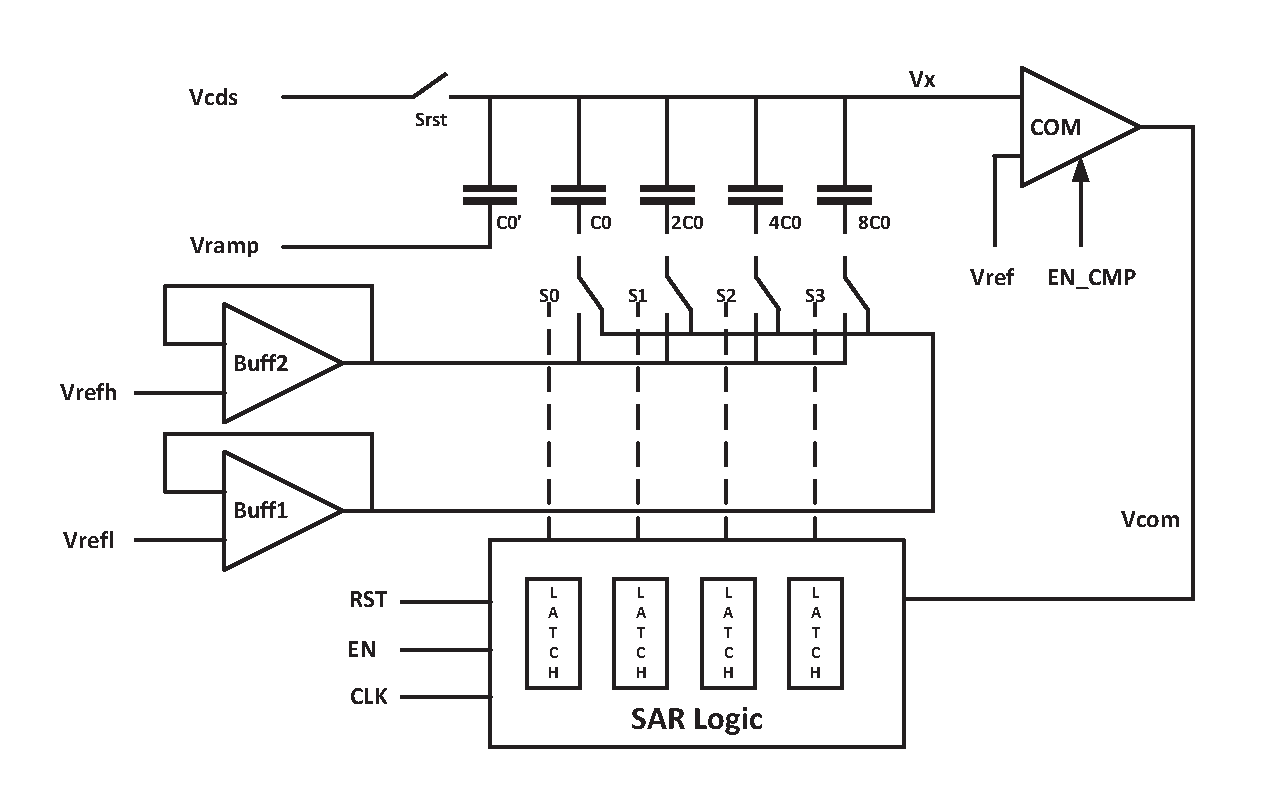
\includegraphics[width=3.5in]{./Figures/SAR.eps}}
	\caption{the Structure of the SAR Sub-ADCs in the SAR/SS ADCs.}
	\label{SAR}
\end{figure} 

\begin{equation}
	V_{X.1}=V_{cds}+\sum_{i=1}^{4} {\frac{V_{ref}}{2^{i}}\ast{D_{U}\left[\,i\,\right]}}
	\label{eq4}
\end{equation}

\begin{equation}
	\begin{aligned}
	&V_{X.2}=V_{X.1}+\frac{V_{ramp}}{2^4}\\ &where\  V_{ramp}=\frac{V_{ref}}{2^6-1}\ast\sum_{i=1}^{6}2^{6-i}\ast{D_{L}\left[\,i\,\right]}
	\label{eq5}
	\end{aligned}	
\end{equation}

\begin{equation}
	\begin{aligned}
	V_{cds}&=k\ast(V_{rst}-V_{sig})\\
	&\;{\approx}\;{V_{ref}-\sum_{i=1}^{4} \frac{V_{ref}}{2^{i}}\ast{D_{U}\left[\,i\,\right]}-\sum_{i=1}^{6} \frac{V_{ref}}{2^{4+i}}\ast{D_{L}\left[\,i\,\right]}}
	\label{eq6}
	\end{aligned}
\end{equation}

\begin{figure}[htbp]
	\centerline{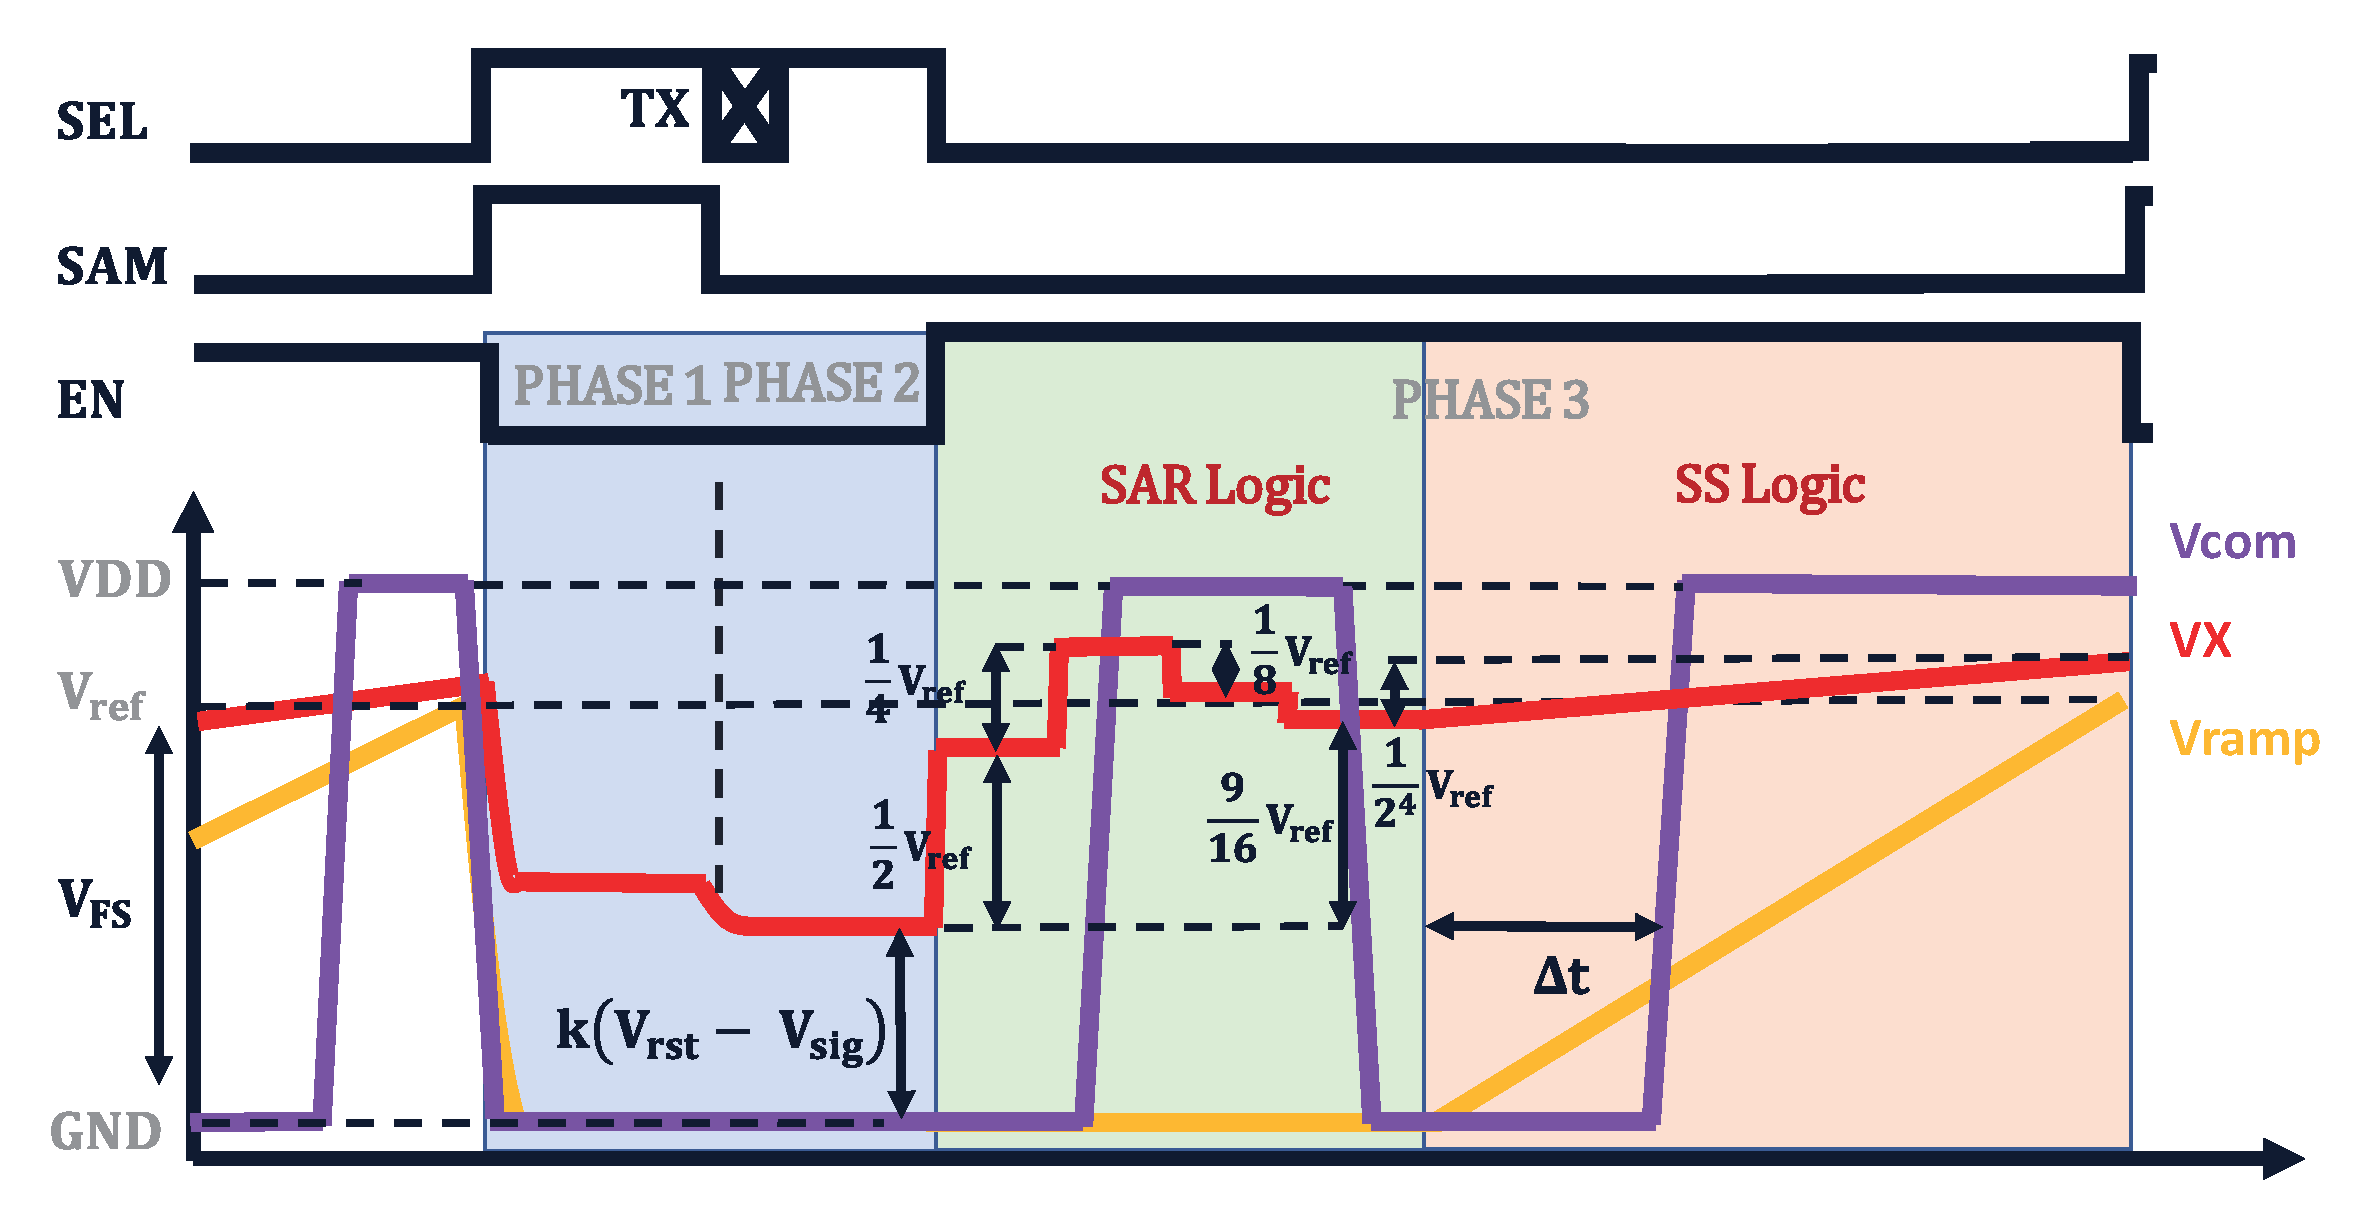
\includegraphics[width=4in]{./Figures/SARWAVE.eps}}
	\caption{the Structure of the SAR Sub-ADCs in the SAR/SS ADCs.}
	\label{SARWAVE}
\end{figure} 

As for the comparators inside the low-precision SAR sub-ADCs, the strong-arm with pre-amp structure is applied, as presented in Fig.~\ref{LATCH}. Such comparators are suitable for multiple comparisons because high speed is easy to achieve. Besides, the pre-amps’ offset voltages can be canceled effectively through the Output Offset Cancelation (OOS) technique [x].

\begin{figure}[htbp]
	\centerline{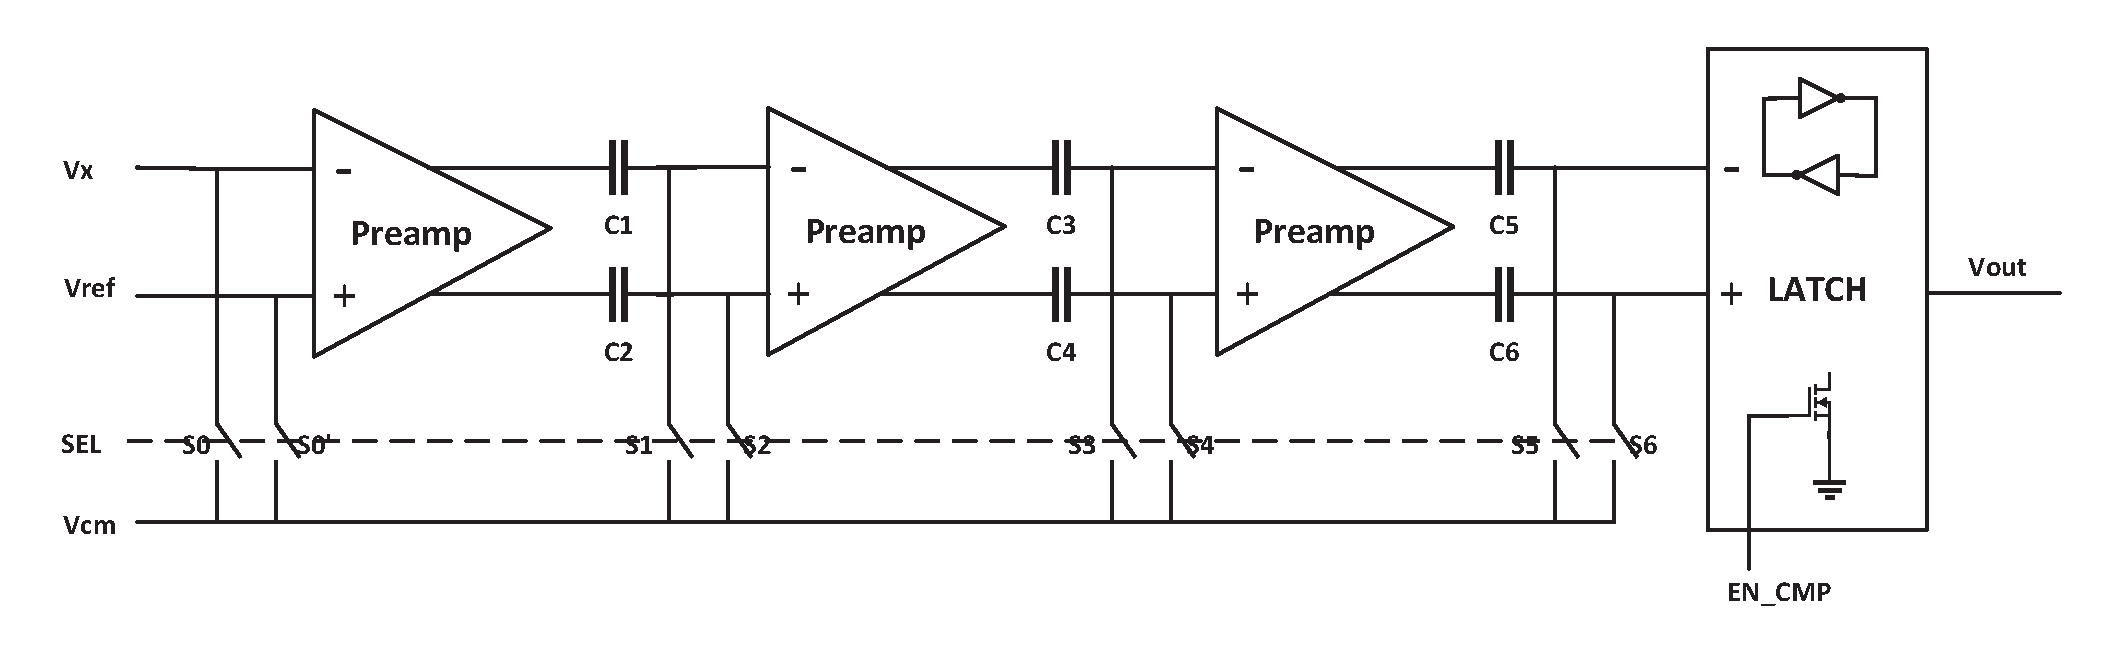
\includegraphics[width=3.5in]{./Figures/LATCH.eps}}
	\caption{the Structure of the Comparators in the SAR Sub-ADCs.}
	\label{LATCH}
\end{figure} 

 The total number of clocks for conversion in the SAR/SS ADCs are 68 ($4+2^6$), which is much less than the SS ADCs where 1024 clocks (for 10 bits) are required. However, the SAR/SS ADCs have traded off area for less conversion clocks. Therefore, for different design specifications, different arcitecture can be chosen.

\section{Adaptive Precision and Power Gating Strategies}\label{strategy}

\subsection{Power Gating Implementation}

The power gating can be implemented simply by adding PMOS-transistor switches between the functional blocks and the supply voltage [x]. When the switches are turned off, the corresponding blocks’ current paths will be cut off, thus the energy is saved. It is obvious that the more currents are under control, the more effective the power gating is. However, to avoid unacceptable IR drop, the total size of the switches will be large, thus inverters should be inserted between the control signal and the switches’ gates for adequate driving capability. Besides, the functional blocks’ recovery speed from power off should be taken into consideration, because the slower the speed is, the less time the blocks can be power gated. 

\subsection{Strategy for the SS ADCs}
As evaluated in Sect.~\ref{result}, the SS ADCs’ power consumption is mainly taken up by the column-parallel comparators, bias circuits, and the output buffer of the ramp generator. Considering that all bias circuits are settled down only once (tens of microseconds after the whole system's power up) and then other circuits can be settled down quickly by the distributed bias circuits, we just apply power gating to the comparators and the output buffer.

The related waveform are presented in Fig.~\ref{SS_pg}. In the low-precision mode, the thermometer counter should have been extended to support switching the capacitors in CDAC 16 by 16 rather than one by one, thus the ramp signal will reach $V_{refh}$ in 16 clocks (for 4 bits) rather than 256 clocks (for 8 bits). After the 16 clocks, the comparators and the output buffer can be power gated for a long time with the output signals drop gradually.

\begin{figure}[htbp]
	\centerline{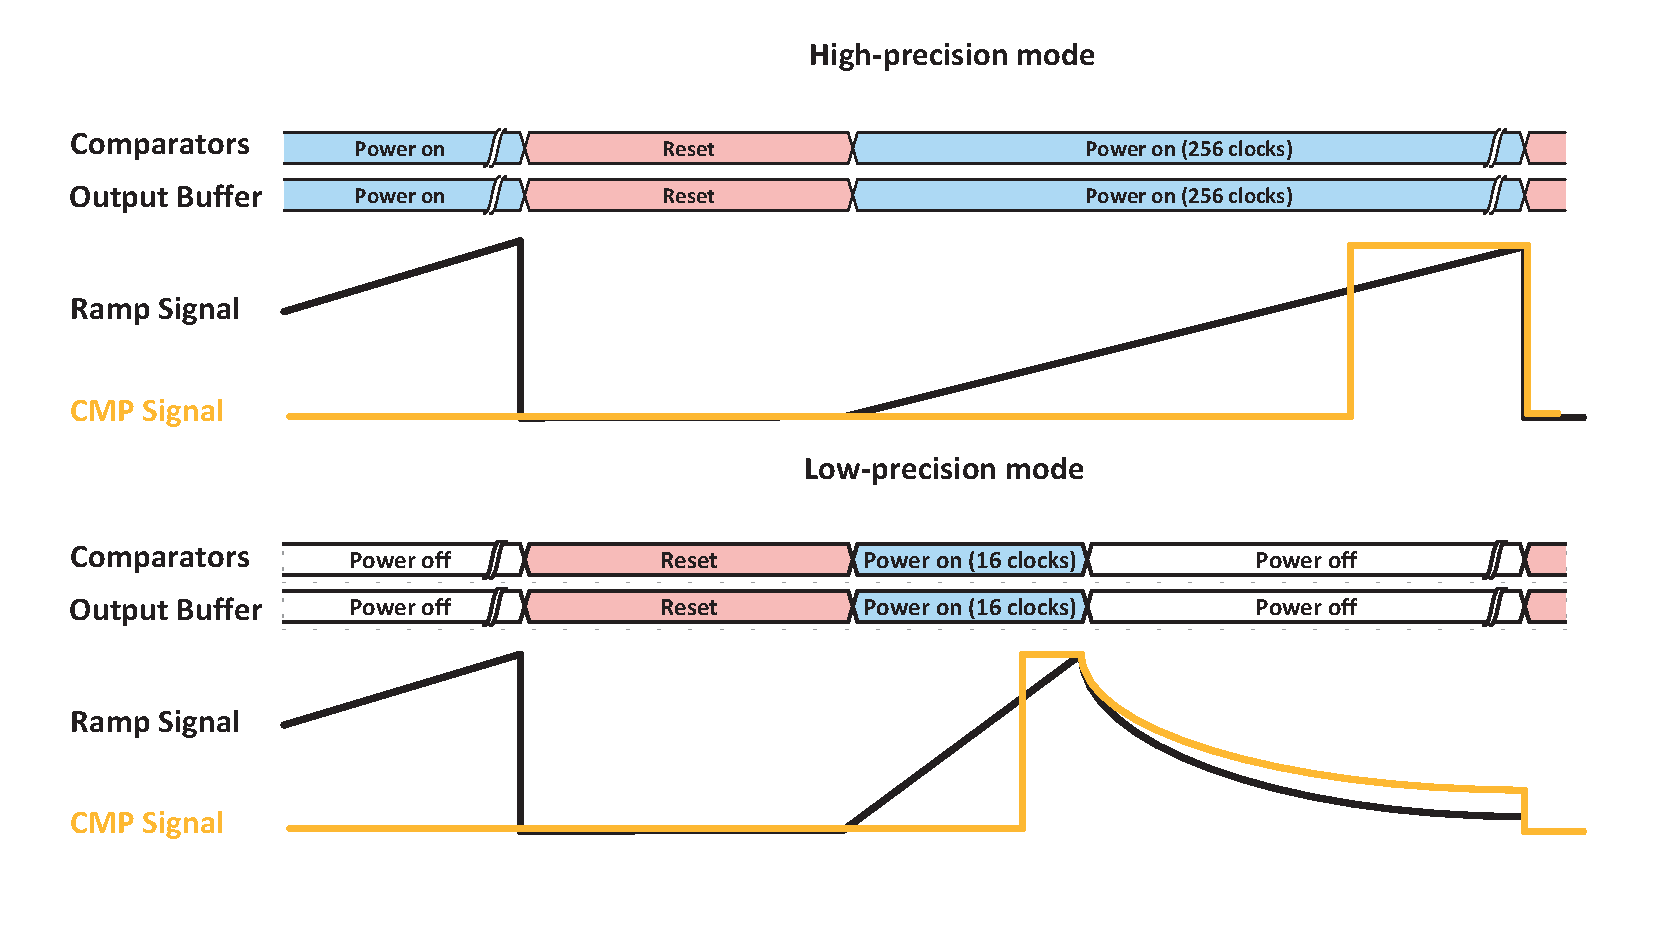
\includegraphics[width=3.5in]{./Figures/SS_pg.eps}}
	\caption{Power Gating and Adaptive Precision Strategies for the SS ADCs.}
	\label{SS_pg}
\end{figure} 

\subsection{Strategy for the SAR/SS ADCs}
As evaluated in Sect.~\ref{result}, the SAR/SS ADCs’ power consumption is mainly taken up by the column-parallel buffers of SAR logic and comparators, which can be power gated with adaptive precision as presented in Fig.~\ref{SAR_pg}. It shows that in the low-precision mode, the ramp signal is generated as usaual but the comparators will be power off then, leaving the 4-bit results converted completely by the SAR logic. 

Compared with the SS ADCs, the thermometer counter in the SAR/SS ADCs does not need to support two modes for adaptive precision. Besides, the start signal of the ramp generator and the power off signal of the comparators can be the same. As for the proportion between the power gating time and the conversion time, 64/68 is achieved in the SAR/SS ADCs, which is similar to the number 240/256 in the SS ADCs.

\begin{figure}[htbp]
	\centerline{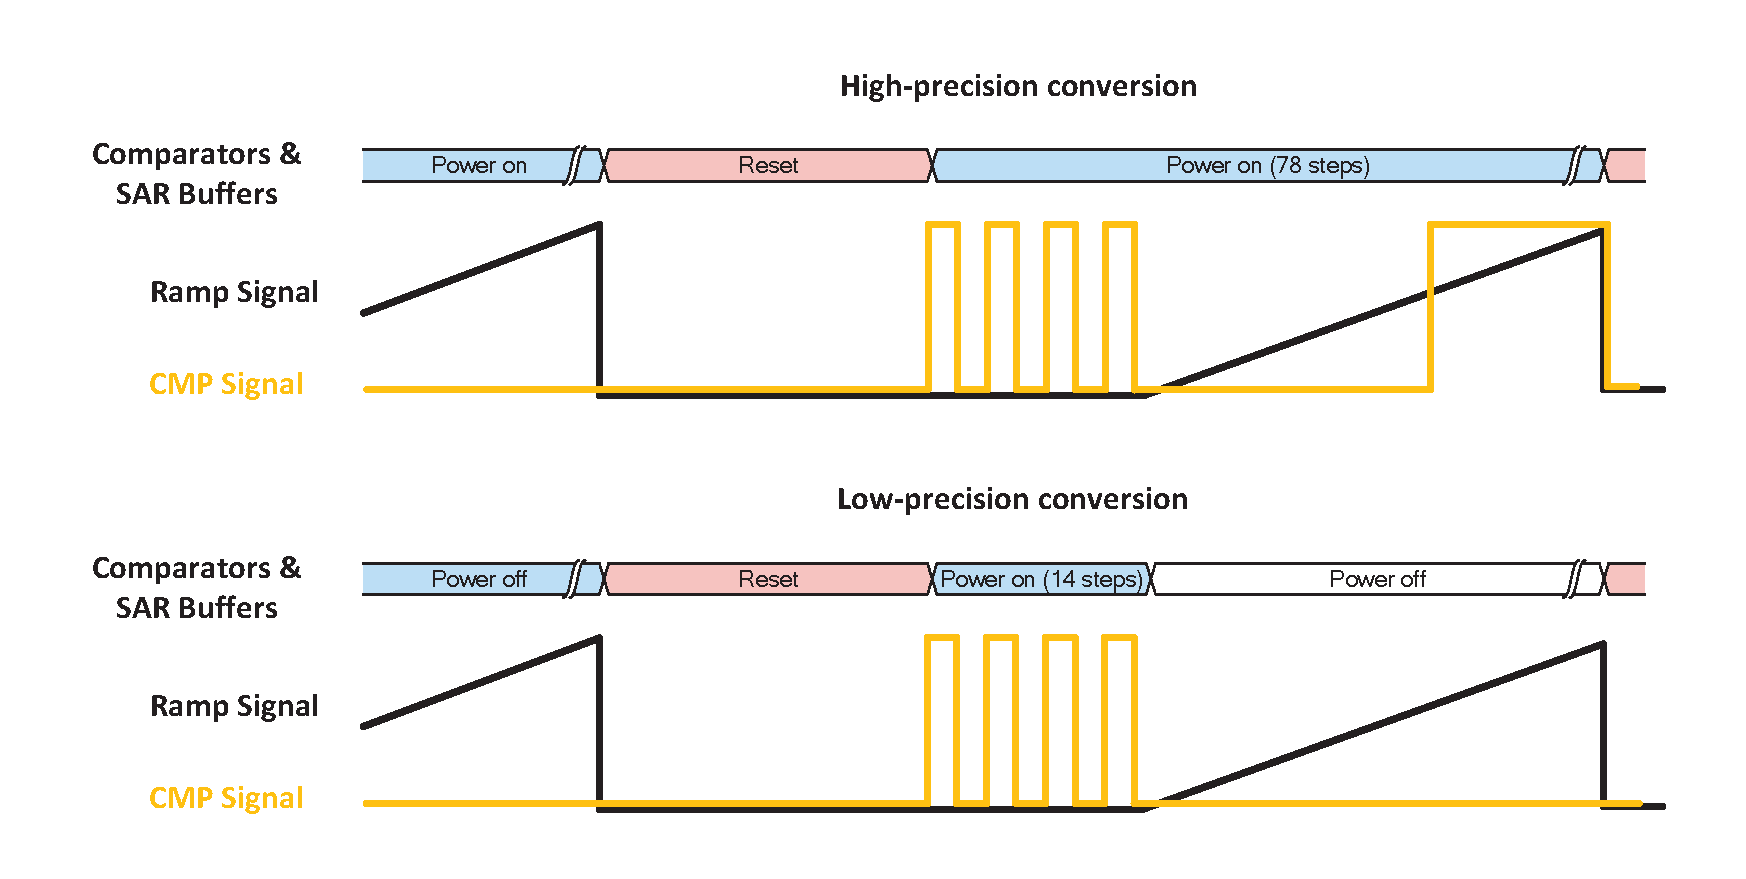
\includegraphics[width=3.5in]{./Figures/SAR_pg.eps}}
	\caption{Power Gating and Adaptive Precision Strategies for the SAR/SS ADCs.}
	\label{SAR_pg}
\end{figure} 

\section{Evaluation Results}\label{result}

This section provides quantitative results of the two case study ADC designs’ fundamental characteristics and energy-saving performance. The statistical data is obtained from simulation in Virtuoso’s AMS Environment. Although some digital modules are in behavior level written by Verilog, we argue that the power consumption of this parts  can be ignored because these digital modules do not have static current paths.

\subsection{Evaluation of the SS ADCs}

The fundamental characteristics of the SS ADCs are summarized in Table~\ref{tab1}. Assuming a 512×512 pixel array, the frame rate will be xx fps. The SNDR of SS ADCs is xx dB/ xx dB, which means the ENOB is 3.x bits/ 7.x bits. The power consumption of the SS ADCs is measured and divided by columns, it shows that compared to xx uW/column in the high-precision mode, only xx uW/column is needed in the low-precision mode, reduced by almost a half. A more specific energy analysis is presented in Fig.~\ref{SSresults1}. As we can see, most parts of the power consumption are taken up by the column-parallel comparators and output buffer of the ramp generator, both of which can be power gated effectively in the low-precision mode. The related quantity results is presented in Fig.~\ref{SSresults2}, where the peripheral circuits include a bandgap and voltage divider, some level-shift circuits and global buffers.
\begin{table}[htbp]
	\caption{Performance of the SS ADCs}
	\begin{center}
		\begin{tabular}{|c|c|}
			\hline
			\textbf{Prameter}& \textbf{Value} \\
			\hhline{|==|}
			\textbf{Process}& 65nm \\
			\hline 
		    \textbf{Supply voltage}& 2.5V/1.2V \\
		    \hline
		    \textbf{Clock Frequency}&	25 MHz \\
		    \hline
		    \textbf{Architecture}&	SS \\
		    \hline
		    \textbf{Quantization bits}&	4/8 \\
		    \hline
		    \textbf{Conversion time (us)}&	2.4 us/12 us \\
		    \hline
		    \textbf{Number of parallel columns}&	512 \\
		    \hline
		    \textbf{Throughput (samples per second)}&	42.7MSPS \\ 
		    \hline
		    \textbf{Power (per column)}&	40.8 uW/76.2 uW \\
		    \hline
		    \textbf{SNDR}& \\
		    \hline
		    \textbf{Fom}& \\
		    \hline	    
		\end{tabular}
		\label{tab1}
	\end{center}
\end{table}
\begin{figure}[htbp]
	\centerline{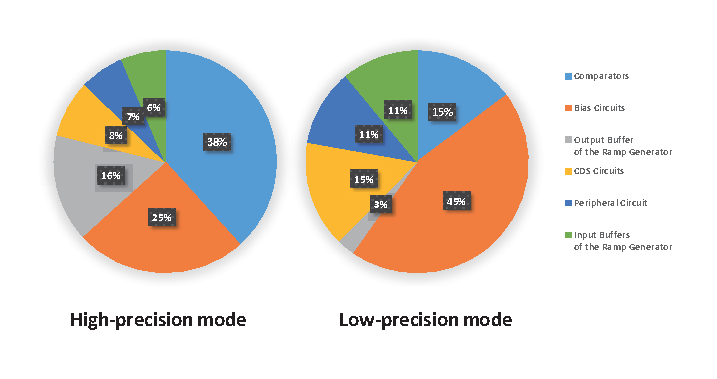
\includegraphics[width=3.5in]{./Figures/SSResults1.eps}}
	\caption{Power Saving Results of the SS ADCs.}
	\label{SSresults1}
\end{figure}
\begin{figure}[htbp]
	\centerline{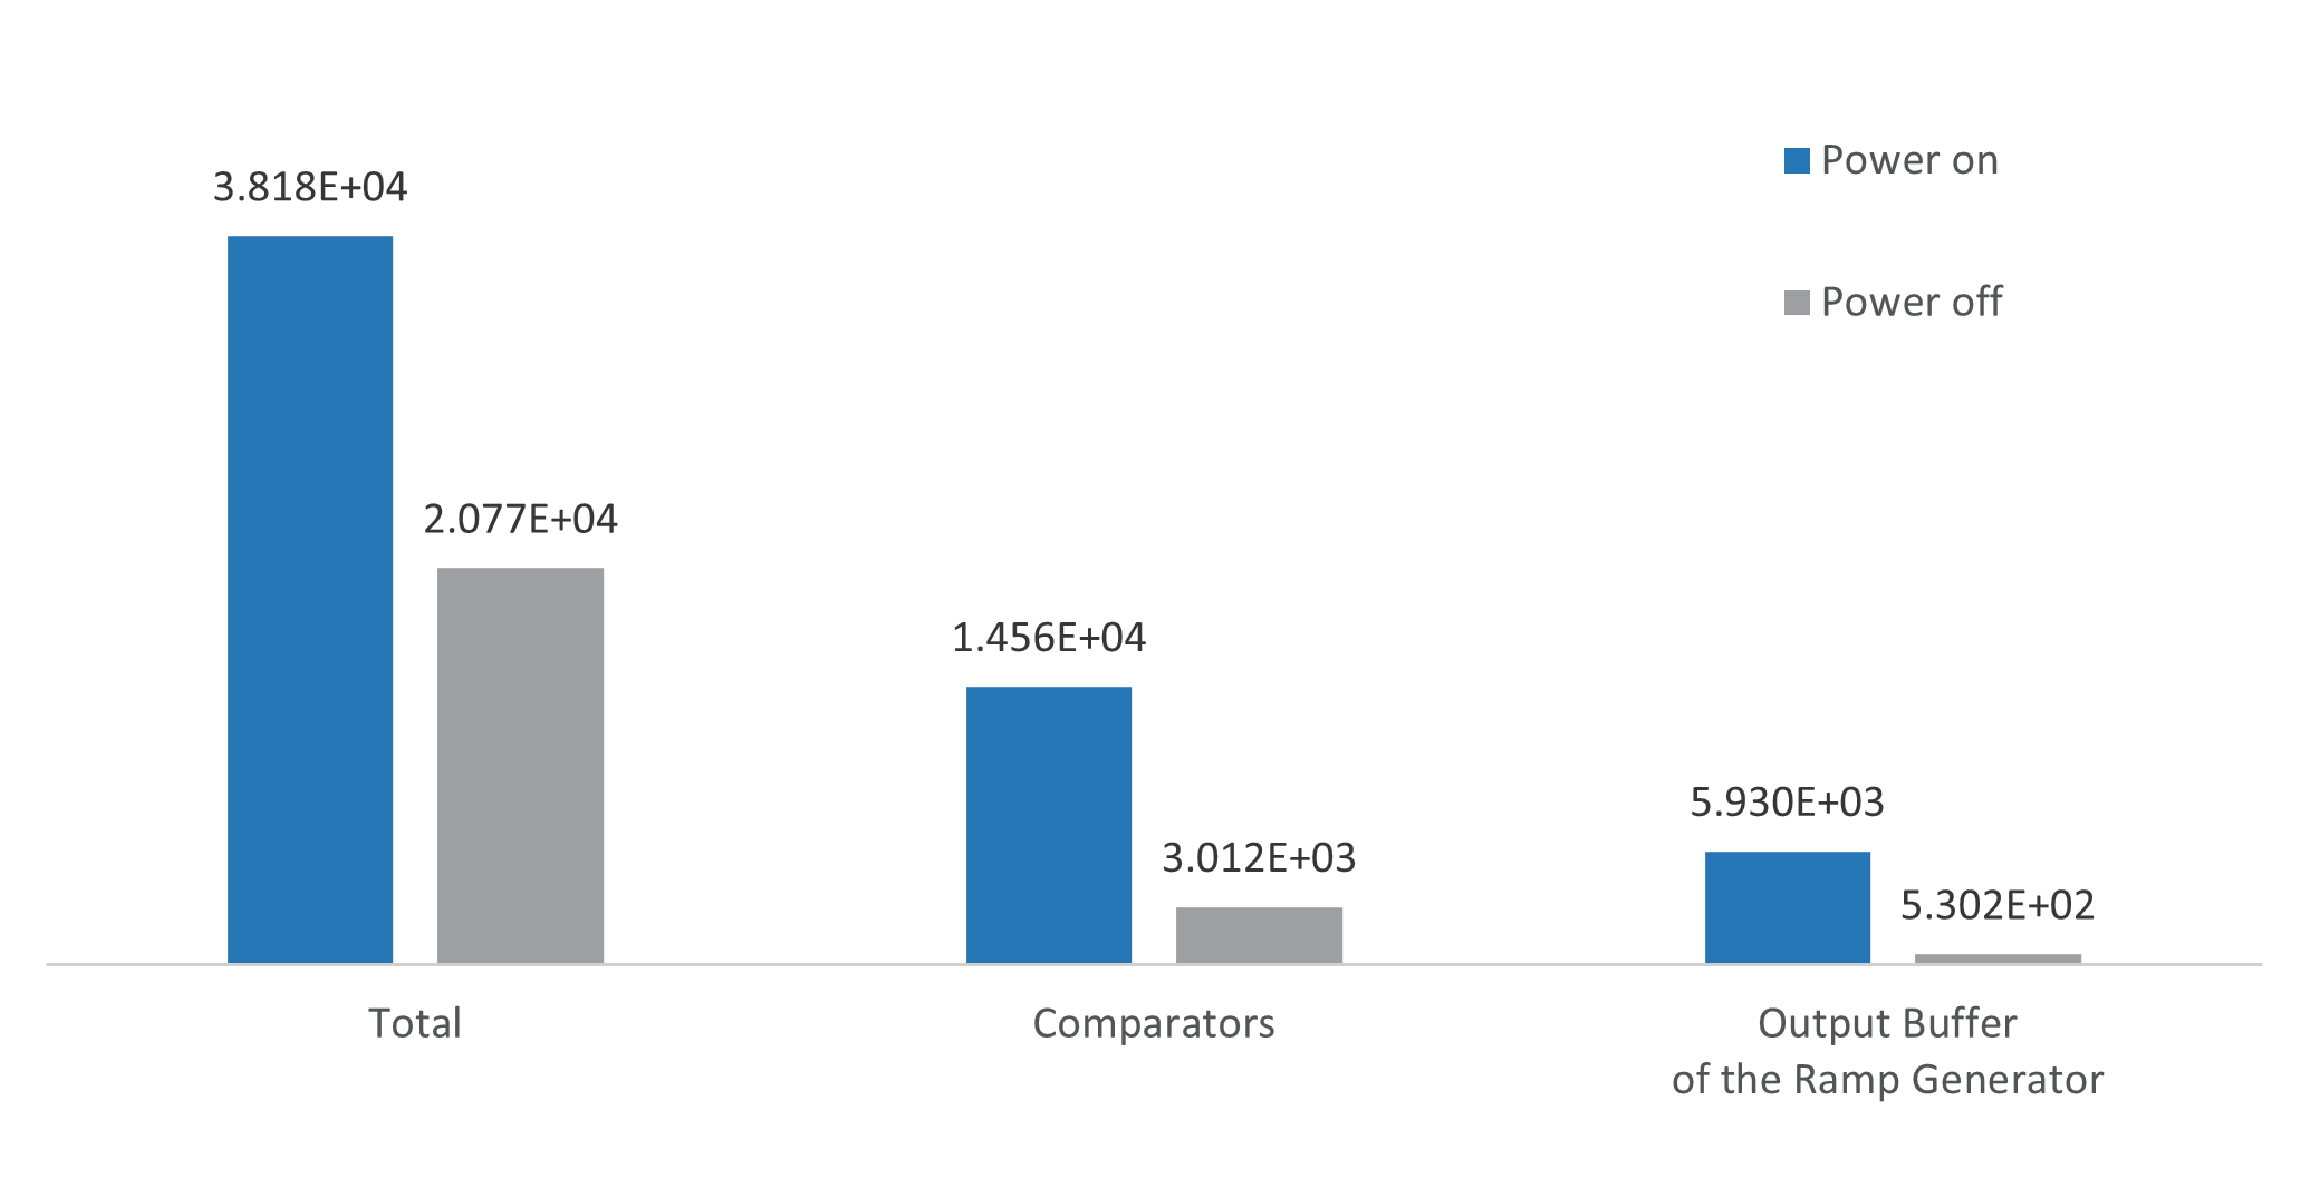
\includegraphics[width=3.5in]{./Figures/SSResults2.eps}}
	\caption{Power Saving Results of the SS ADCs.}
	\label{SSresults2}
\end{figure} 

\subsection{Evaluation of the SAR/SS ADCs}
The fundamental characteristics of the SAR/SS ADCs are summarized in Table~\ref{tab2}. While the throughput is set similar to the SS ADCs, a lower clock frequency is required. The SNDR is xx dB/ xx dB and the ENOB is 3.x bits/ 9.x bits, consistent with the design specifications. The power consumption is xx uW/column in the high-precision mode and xx uW/column in the low-precision mode, respectively. According to the energy analysis presented in Fig.~\ref{SARresults1}, most parts of the SAR/SS ADCs' power consumption are taken up by the column-parallel comparators and buffers of SAR logic. And in the low-precision mode, this parts' energy can also be reduced to nearly half. The related quantity results is presented in Fig.~\ref{SARresults2}.
\begin{table}[htbp]
	\caption{Performance of the SAR/SS ADCs}
	\begin{center}
		\begin{tabular}{|c|c|}
			\hline
			\textbf{Prameter}& \textbf{Value} \\
			\hhline{|==|}
			\textbf{Process}& 65nm \\
			\hline 
			\textbf{Supply voltage}& 2.5V/1.2V \\
			\hline
			\textbf{Clock Frequency}&	25 MHz \\
			\hline
			\textbf{Architecture}&	SS \\
			\hline
			\textbf{Quantization bits}&	4/8 \\
			\hline
			\textbf{Conversion time (us)}&	2.4 us/12 us \\
			\hline
			\textbf{Number of parallel columns}&	512 \\
			\hline
			\textbf{Throughput (samples per second)}&	42.7MSPS \\ 
			\hline
			\textbf{Power (per column)}&	40.8 uW/76.2 uW \\
			\hline
			\textbf{SNDR}& \\
			\hline
			\textbf{Fom}& \\
			\hline	    
		\end{tabular}
		\label{tab2}
	\end{center}
\end{table}
\begin{figure}[htbp]
	\centerline{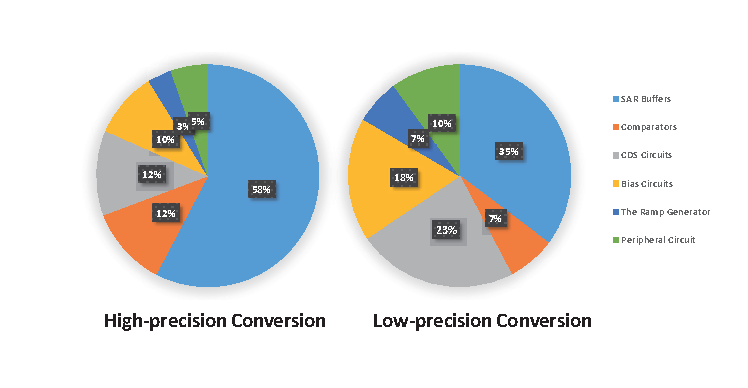
\includegraphics[width=3.5in]{./Figures/SARResults1.eps}}
	\caption{Power Saving Results of the SAR/SS ADCs.}
	\label{SARresults1}
\end{figure} 
\begin{figure}[htbp]
	\centerline{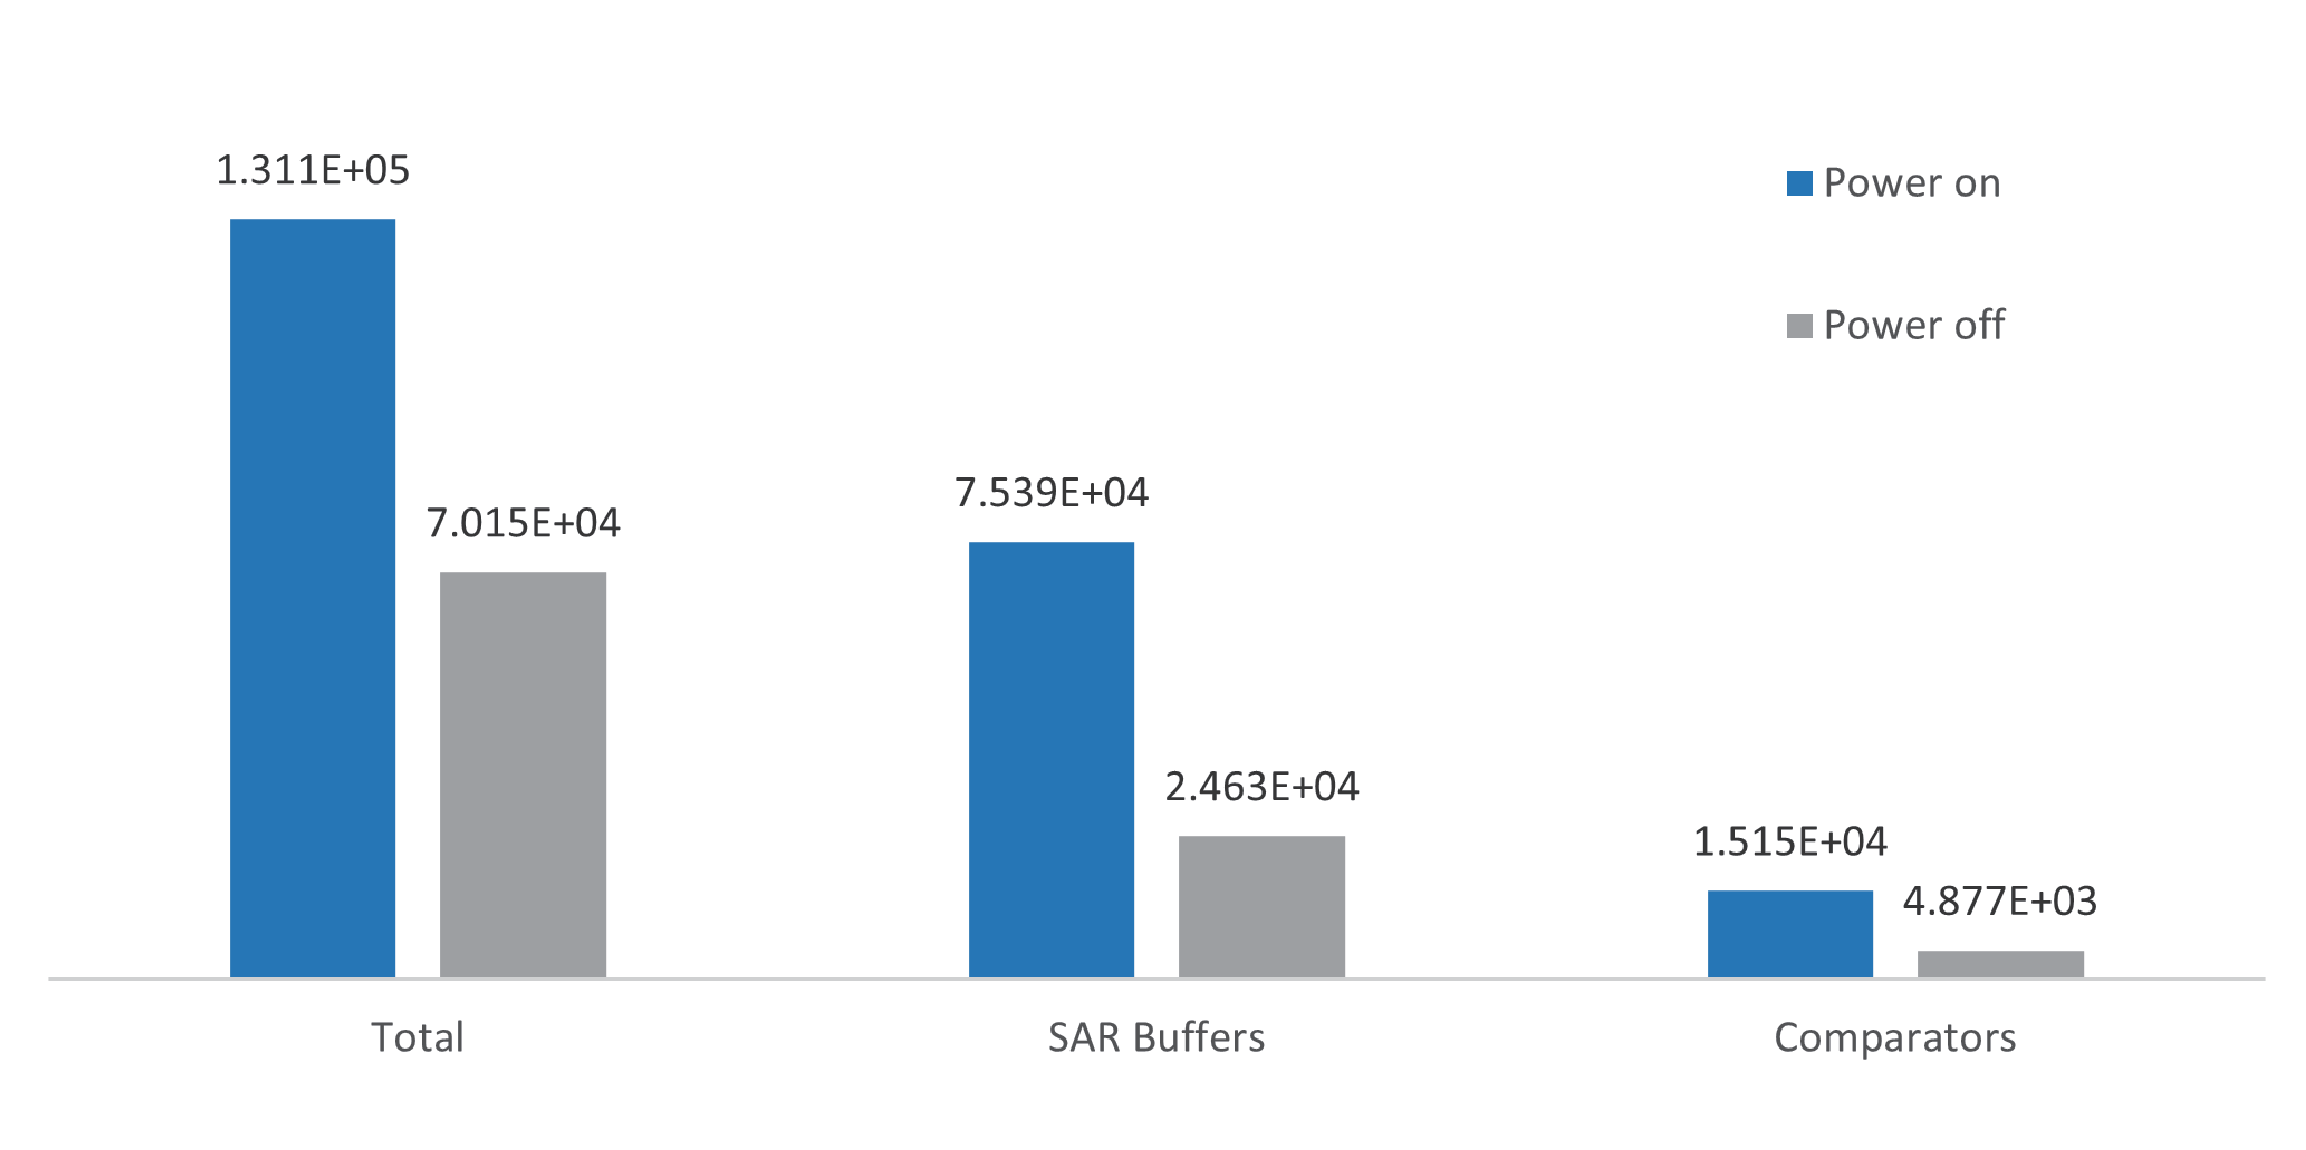
\includegraphics[width=3.5in]{./Figures/SARResults2.eps}}
	\caption{Power Saving Results of the SAR/SS ADCs.}
	\label{SARresults2}
\end{figure} 

\section{Discussions}\label{discussion}
With precision adaptive and power gating strategies, both the SS ADCs and SAR/SS ADCs can save energy dynamically and significantly. 

In comparison, the SAR/SS ADCs can support higher quantization bits and require fewer extra control circuits for the adaptive precision, while SS ADCs inherently require less area and can effectively applied in the 4/8-bit situation. Therefore, according to specific design specifications, different structures can be chosen. 

For other different precision configurations (e.g. 2/8 adaptive precision) and number of parallel collumns, the corresponding power consumption and energy-saving performance can also be estimated with extending the evaluation results in Sect.~\ref{result}. 

\section{Conclusions}\label{conclusion}

In this work, a method combining adaptive precision with power gating is proposed for more smart ADCs' design with dynamicall energy optimization. According to the evaluation results of two CIS-applied ADC designs, almost a half of the ADCs’ power consumption can be reduced in the low precision mode, while the cost of extra control circuits is rather small.

 The method in this paper is universal and has prospects to be combined with varying downstream intelligent algorithms for efficient multi-tasks analysis. As such an integrated system will be more promising for edge computing in the future, more works on the co-design of ADCs and algorithms remain to be developed.

\begin{thebibliography}{00}
\bibitem{b1} G. Eason, B. Noble, and I. N. Sneddon, ``On certain integrals of Lipschitz-Hankel type involving products of Bessel functions,'' Phil. Trans. Roy. Soc. London, vol. A247, pp. 529--551, April 1955.
\bibitem{b2} J. Clerk Maxwell, A Treatise on Electricity and Magnetism, 3rd ed., vol. 2. Oxford: Clarendon, 1892, pp.68--73.
\bibitem{b3} I. S. Jacobs and C. P. Bean, ``Fine particles, thin films and exchange anisotropy,'' in Magnetism, vol. III, G. T. Rado and H. Suhl, Eds. New York: Academic, 1963, pp. 271--350.
\bibitem{b4} K. Elissa, ``Title of paper if known,'' unpublished.
\bibitem{b5} R. Nicole, ``Title of paper with only first word capitalized,'' J. Name Stand. Abbrev., in press.
\bibitem{b6} Y. Yorozu, M. Hirano, K. Oka, and Y. Tagawa, ``Electron spectroscopy studies on magneto-optical media and plastic substrate interface,'' IEEE Transl. J. Magn. Japan, vol. 2, pp. 740--741, August 1987 [Digests 9th Annual Conf. Magnetics Japan, p. 301, 1982].
\bibitem{b7} M. Young, The Technical Writer's Handbook. Mill Valley, CA: University Science, 1989.
\end{thebibliography}

\end{document}
